\documentclass{article}
\usepackage[utf8]{inputenc}
\usepackage{subcaption}
\usepackage{amsmath}
\usepackage{amssymb}
\usepackage{hyperref}
\usepackage{titlesec}
\usepackage{xcolor}
\usepackage{csquotes}
\usepackage{fancyhdr}
\usepackage{graphicx}
\usepackage{listings}
\usepackage{multirow}
\usepackage{wrapfig}
\usepackage[backend=biber,style=numeric,sortcites,natbib=true,sorting=none]{biblatex}
\addbibresource{report.bib}
\usepackage{enumitem}
\usepackage[rightcaption]{sidecap}
\usepackage{verbatim}
\usepackage[backend=bibtex]{biblatex}
\usepackage [ a4paper , hmargin =1.2 in , bottom =1.5 in ] { geometry }
\usepackage{xcolor}
\definecolor{lightgray}{rgb}{0.95, 0.95, 0.95}
\definecolor{darkgray}{rgb}{0.4, 0.4, 0.4}
\definecolor{purple}{rgb}{0.65, 0.12, 0.82}
\definecolor{editorGray}{rgb}{0.95, 0.95, 0.95}
\definecolor{editorOcher}{rgb}{1, 0.5, 0} % #FF7F00 -> rgb(239, 169, 0)
\definecolor{editorGreen}{rgb}{0, 0.5, 0} % #007C00 -> rgb(0, 124, 0)
\definecolor{orange}{rgb}{1,0.45,0.13}		
\definecolor{olive}{rgb}{0.17,0.59,0.20}
\definecolor{brown}{rgb}{0.69,0.31,0.31}
\definecolor{purple}{rgb}{0.38,0.18,0.81}
\definecolor{lightblue}{rgb}{0.1,0.57,0.7}
\definecolor{lightred}{rgb}{1,0.4,0.5}
\definecolor{codegreen}{rgb}{0,0.6,0}
\definecolor{codegray}{rgb}{0.5,0.5,0.5}
\definecolor{codepurple}{rgb}{0.58,0,0.82}
\definecolor{backcolour}{rgb}{0.95,0.95,0.92}
\hypersetup{
    colorlinks=true,
    linkcolor=blue,
    filecolor=magenta,      
    urlcolor=cyan,
}
\lstdefinestyle{mystyle}{
    backgroundcolor=\color{backcolour},   
    commentstyle=\color{codegreen},
    keywordstyle=\color{magenta},
    numberstyle=\tiny\color{codegray},
    stringstyle=\color{codepurple},
    basicstyle=\ttfamily\footnotesize,
    breakatwhitespace=false,         
    breaklines=true,                 
    captionpos=b,                    
    keepspaces=true,                 
    numbers=left,                    
    numbersep=5pt,                  
    showspaces=false,                
    showstringspaces=false,
    showtabs=false,                  
    tabsize=2
}
%CSS 
\lstdefinelanguage{CSS}{
  keywords={margin:,padding:,display:,flex-direction:,justify-content:,align-items:,background-color:,height:,font-family:,margin-bottom:,text-shadow:,font-size:,position:,text-align:,border-radius:,box-shadow:,grid-template-columns:,grid-gap:,width:,align-content:,border:,cursor:,line-height:,transform:,pointer-events:,animation:,margin-right:,margin-top:,color:,top:,left:,right:,opacity:,transition:,z-index:,},	
  sensitive=true,
  morecomment=[l]{//},
  morecomment=[s]{/}{/},
  morestring=[b]',
  morestring=[b]",
  alsoletter={:},
  alsodigit={-}
}

% JavaScript
\lstdefinelanguage{JavaScript}{
  morekeywords={typeof, new, true, false, catch, function, return, null, catch, switch, var, if, in, while, do, else, case, break, let, const, event},
  morecomment=[s]{/}{/},
  morecomment=[l]//,
  morestring=[b]",
  morestring=[b]'
}

\lstset{style=mystyle}
\pagestyle{fancy}
\fancyhf{}
\lhead{Minesweeper Cricket}
\rhead{Sanoj S Vijendra}
\cfoot{Page \thepage}

\title{Minesweeper Cricket}
\author{Sanoj S Vijendra}
\date{June 2023}

\begin{document}

\maketitle

\tableofcontents
\clearpage

\section{Introduction}
Introducing "Minesweeper Cricket," a captivating fusion of the classic Minesweeper game and the excitement of cricket. Uncover hidden runs on a grid while strategically avoiding fielders to score as many runs as possible before running out of wickets. With varying grid sizes, live score display, reveal options, and a leader-board, this game offers an addictive blend of strategic thinking and cricket thrills for players of all ages. Immerse yourself in the world of "Minesweeper Cricket" and aim for the highest score in this innovative twist on a beloved classic.
\section{Customisation}
\subsection{Feel of Cricket}
This game evokes the excitement and thrill of cricket by incorporating elements from the sport into its gameplay. \\
\begin{itemize}
\item As players uncover hidden runs on the grid, they experience the same anticipation and strategic decision-making that cricketers face on the field.
\item There are hidden fielders present on the playing field randomly, if user clicks on them, he gets out just same as in actual cricket (when you attempt to smash a ball and find a fielder you get out).
\item The game's immersive environment, coupled with live score updates and leaderboard rankings, creates a sense of competition and engagement akin to a real cricket match. 
\end{itemize}
\begin{figure}[h!]
    \centering
    \begin{subfigure}[c]{0.49\textwidth}
        \centering
        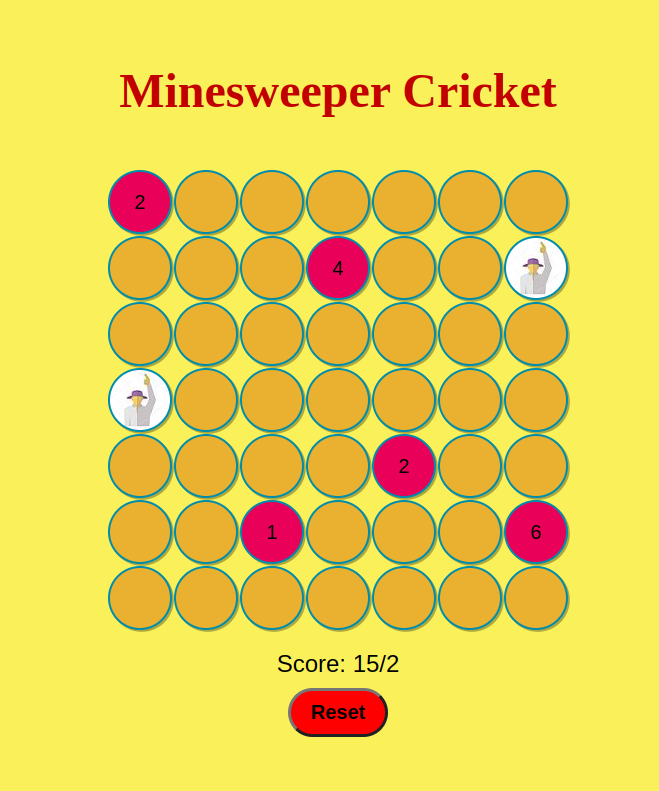
\includegraphics[width=1\textwidth]{board.png}
        \caption{Game Board}
        \label{1a}
    \end{subfigure}
\end{figure}
\subsection{Grid-Size}
This game allow user to select the appropriate grid size of his choice among 5x5, 6x6, 7x7, 8x8 and 9x9. \autocite{1}
\begin{enumerate}
\item \texttt{[5 x 5]}: Number of fielders present on the field are 5 and user has 3 wickets.
\item \texttt{[6 x 6]}: Number of fielders present on the field are 6 and user has 4 wickets.
\item \texttt{[7 x 7]}: Number of fielders present on the field are 9 and user has 5 wickets.
\item \texttt{[8 x 8]}: Number of fielders present on the field are 11 and user has 5 wickets.
\item \texttt{[9 x 9]}: Number of fielders present on the field are 11 and user has 5 wickets.
\end{enumerate}
\subsection{Power Ups}
\begin{itemize}
\item {\bfseries Multiple Runs:} User can score more than singles by clicking on the grids. Runs present on the board are generated randomly. Runs which can be scored are 1,2,3,4 and 6. Probability of hitting sixes is around \textbf{1/3 !}.
\item {\bfseries Revealing Fielders:} If a players makes four successful moves without getting out then he is rewarded with a power up which will reveal the location of a fielder placed on the board randomly for 1 or 2 seconds. But there is also a catch with this. So, be wise to while using this feature.
\end{itemize}
\begin{figure}[h!]
    \centering
    \begin{subfigure}[c]{0.49\textwidth}
        \centering
        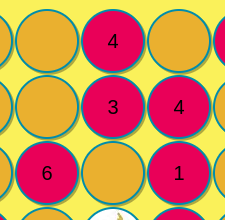
\includegraphics[width=1\textwidth]{runs.png}
        \caption{Runs}
        \label{2}
    \end{subfigure}
    \hfill
    \begin{subfigure}[c]{0.49\textwidth}
        \centering
        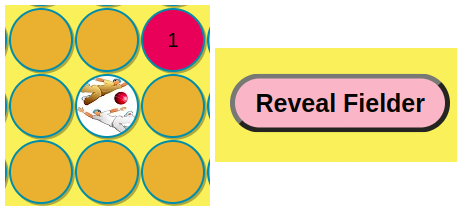
\includegraphics[width=1\textwidth]{reveal_fielder.png}
        \caption{Fielders}
        \label{2}
    \end{subfigure}
\end{figure}
\newpage
\subsection{Leaderboard}
\begin{wrapfigure}[10]{r}{0.4\textwidth}
  \vspace{-1.5\baselineskip}
  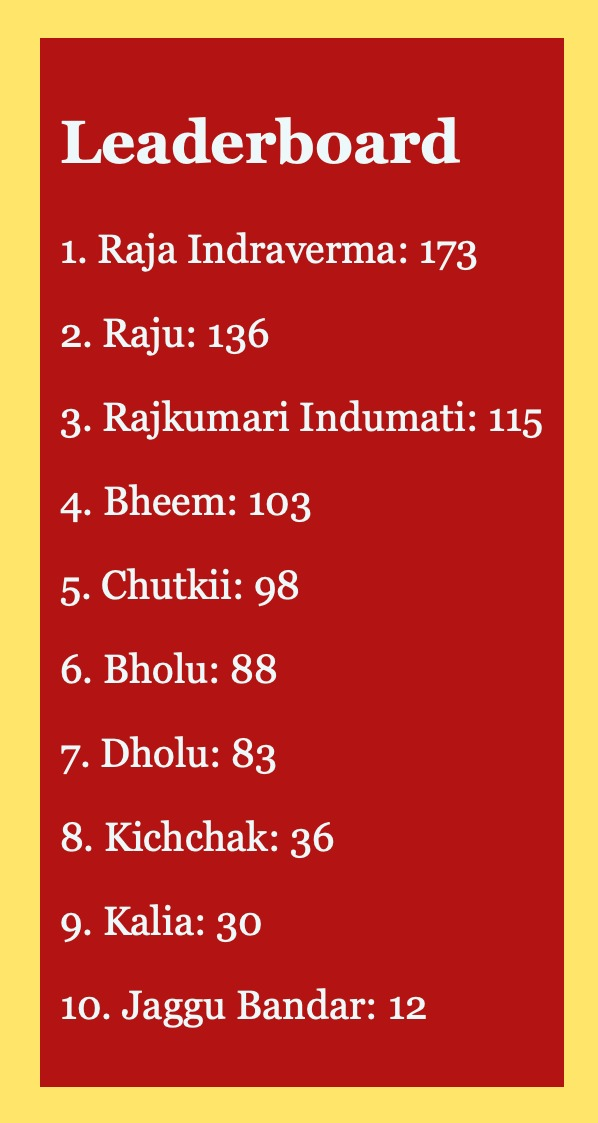
\includegraphics[width=0.8\linewidth, valign=t]{leaderboard.png}
\end{wrapfigure}
The leaderboard in adds an extra layer of competitiveness and motivation for players. It showcases the top performers, allowing them to compare their scores and achievements with other players. By achieving higher scores and completing levels with efficiency, players can climb up the leaderboard. With real-time updates and a ranking system, the leaderboard in the game adds a dynamic and interactive element to the game.
\\
\\
\\
\\
\\
\\
\\
\\
\\
\\
\section{CSS}
In this section, I will explain the CSS I have used. \autocite{2}
\subsection{Colors}
The page layout is extensively designed for visual appeal using CSS. A combination of shades of red, orange and yellow is used to bring about contrast and make the color pallet look beautiful. Apart from this different hover colors are added on buttons.
\subsection{Buttons}
\begin{enumerate}
\item {\bfseries Grid Size Button:} Initially button has rounded edge and have background color of pink. When user hover over the button, it will undergo a 360\textdegree{} rotation about X-axis and its color will change to blue in about 0.7 seconds to give a smooth transition. Also, inside text color will change to white. Additionally, a blurry shadow will be produced.
\item {\bfseries Instruction/Hide:} Initially button has background color orange but when user hover over it, its color will change to green and its size will be scaled 1.1 times of original in about 1 second to give a smooth transition. Color of inside text will change from black to white. Also, "instructions" written on it changes to "hide" and vice-versa. Additionally, a blurry shadow will be produced.
\item {\bfseries Start/Reset:} Initially button has background color of red but when user hover over it, its color will change to blue and its size will be scaled 1.1 times of original in about 1 second to give a smooth transition. Color of inside text will change from black to white.  Additionally, a blurry shadow will be produced.
\item {\bfseries Reveal Fielder:} This button when appears, start to blink with a time period of 1 second. Initially, it has background color of pink. On hovering over it, blinking stops and backgound color changes to blue. Color of text changes from black to white. This all takes about 1 second time which will give it a smooth transition. Additionally, a blurry shadow will be produced.
\end{enumerate}
\subsection{Grid}
The shape of the grid tiles is changed from the traditional square to circle by changing the border percentage. Also, each of the grid has a shadow following it. Whenever a tile is clicked, it undergoes a 360\textdegree{} rotation about the Y-axis. If clicked tile has no fielder on it, the tile will become pinkish (intially orange) and run which is scored will be displayed on it. Else if, there is a fielder, the tile will show a picture of umpire showing the out signal.
\subsection{Reveal Fielder}
When "Reveal Fielder" button is clicked then randomly a tile is selected which have hidden fielder and it will change into a figure having fielder inside it for 1 second then return to original color.
\subsection{Instruction Box}
It is shown when instruction button is clicked and hides when hide button is clicked. When user hover over the instruction button it will scale to 1.1 times of its size in about 1 second to give a soomth transition effect. Additionally, a blurry shadow of the box will be produced.
\subsection{Leaderboard Table}
It is shown at the end of the game. It has background color brown and text color white. On hovering over it, it gets scaled to its 1.1 times of its original size in about 1 second to give a smooth transition effect. Additionally, a blurry shadow of the box will be produced.
\subsection{Miscellaneous}
The game tile has red-orange color and score section had black color. Font of all texts are Times New Roman.
\section{JavaScript}
in this section JS code of the game will be explained, especially different functions used. \autocite{3}
\begin{itemize}
\item  \textbf{toggleInstructions():} This function is responsible for toggling the visibility of an \textit{instructions} div and updating the text from "Instructions" to "Hide" of the corresponding button. 
\item \textbf{setGridSize(size):} This function is responsible for setting the grid size and adjusting the game elements accordingly. The function takes a parameter 'size' which represents the desired grid size. This function also sets the number wickets corresponding to the grid size.
\item \textbf{createGrid():} This function is responsible for dynamically creating a grid of blocks based on a selected grid size.
\item \textbf{generateFielders():} This function is responsible for randomly generating the locations of fielders on the game-board according to the grid size.
\item \textbf{startGame():} This function is called when start("Are You Ready!") button is clicked. This will initiate the game and set up the initial game state. Additionally, it calls \textit{createGrid()}, \textit{generateFielders()} and \textit{loadLeaderboard()} functions within itself.
\item \textbf{blockClick(event):} This function initially checks if /textit{gameOver} is true or not. If not, it will increment \textit{successfulMoves} variable and then checks if it is divisible by 5 or not. If it is divisible, then it will activate "Reveal Fielder" button until user does not click it or he loses a wicket. It then checks, if the clicked tile contains fielder or not. If it has fielder, then it checks the number of wicket fell and calls \textit{wicketfall()} or \textit{displayGameOver()} and \textit{updateLeaderboard()} functions accordingly. This function also assign random runs to the tiles based on assigned probability. It also updates the total score of the user. This function is also responsible for assigning rotating animation to the tile when it is clicked.
\item \textbf{revealFielder():} This function is called when "Reveal Fielder" button is clicked. It reveals a randomly chosen fielder on the grid for a short duration.
\item \textbf{wicketfall():} This function is called when a tile containing fielder is clicked, indicating that a wicket has fallen. It updates the \emph{wickets, lives} and \emph{successfulMoves} variable accordingly and hides the "Reveal Button". It then displays an alert box showing that wicket has fallen.
\item \textbf{resetGame():} This function is called when the player clicks "Reset Button". This function resets the game and takes user to home screen.
\item \textbf{displayGameOver():} This function is called when user loses all its wickets. It displays an alert box showing game over and showing final score of user. Then it calls the function \emph{promptPlayerName()} and \emph{displayLeaderboard()}.
\item \textbf{loadLeaderboard():} This function is responsible for loading the leaderboard data from the browser's local storage and updating the leaderboard display by calling \emph{updateLeaderboard()} function.
\item \textbf{addToLeaderboard():} This function is responsible for adding the current player's data to the leaderboard and storing it in the browser's local storage. It also checks the number of entries already in leaderboard. If it is greater than 10 then it compares new added score and sort the whole leaderboard in descending order. Then it truncates its number of entries to 10.
\item \textbf{displayLeaderboard():} This function is responsible for rendering the leaderboard on the webpage.
\end{itemize}
\clearpage
\section{Source Code}
\subsection{HTML}
\lstinputlisting[language=HTML]{board.html}
\subsection{CSS}
\lstinputlisting[language=CSS]{style.css}
\subsection{JavaScript}
\lstinputlisting[language=JavaScript]{script.js}
\printbibliography
\end{document}
